\documentclass[tikz,border=5mm,12pt]{standalone}
\usetikzlibrary{backgrounds}

\begin{document}
  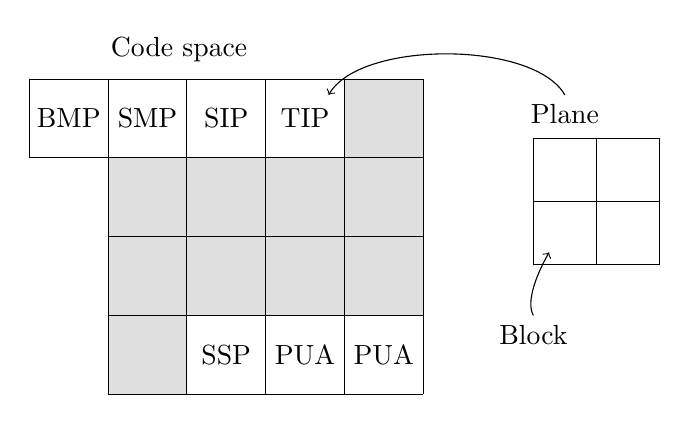
\begin{tikzpicture}
    \draw[step=10mm] (0,0) grid (40mm,40mm);
    \draw (0,40mm) -- ++(-10mm,0) -- ++(0,-10mm) -- ++(10mm,0);

    \node[above] at (9mm,41mm) {Code space};

    \node at (-5mm,35mm) {BMP};
    \node at (5mm,35mm) {SMP};
    \node at (15mm,35mm) {SIP};
    \node at (25mm,35mm) {TIP};
    \node at (15mm,5mm) {SSP};
    \node at (25mm,5mm) {PUA};
    \node at (35mm,5mm) {PUA};

    \begin{scope}[on background layer]
      \path[fill=lightgray!50]
        (0,0)
        -- ++(10mm,0)
        -- ++(0,10mm)
        -- ++(30mm,0)
        -- ++(0,30mm)
        -- ++(-10mm,0)
        -- ++(0,-10mm)
        -- ++(-30mm,0)
        -- cycle;
    \end{scope}

    \draw[<-] (28mm,38mm) .. controls +(60:8mm) and +(120:8mm) .. ++(30mm,0) node[below] {Plane};

    \draw (54mm,32.5mm) -- ++(16mm,0) -- ++(0,-16mm) -- ++(-16mm,0) -- cycle;
    \draw (54mm+8mm,32.5mm) -- ++(0,-16mm);
    \draw (54mm+16mm,32.5mm-8mm) -- ++(-16mm,0);

    \draw[<-] (56mm,18mm) .. controls +(-120:3mm) and +(120:2mm) .. ++(-2mm,-8mm) node[below] {Block};
  \end{tikzpicture}
\end{document}
